\section{Un protocole d'échantillonnage aléatoire adaptatif}

\begin{frame}{Communication}{Contexte Web}

  \large
  \begin{itemize}
  \item [$\Rightarrow$] \textbf{Le protocole de construction du réseau doit
      pouvoir supporter un nombre fluctuant d'utilisateurs ET les standards des
      navigateurs Web.}
  \end{itemize}

  \vspace{1cm}

  \begin{center}
    
\includegraphics[width=0.2\textwidth]{img/webrtc.png}
  \end{center}

\end{frame}


\begin{frame}{Communication}{État de l'art}

  \begin{center}
    \begin{table}[H]
      
\small
\begin{tabularx}{0.5\textwidth}{@{}ccc@{}}
  \toprule 
  \textsc{Protocole} & \textsc{Adaptatif} & \textsc{Web} \\ \midrule
  \CYCLON\footfullcite{voulgaris2005cyclon} & \NO{\xmark} & \YES{\cmark} \\
  \SCAMP\footfullcite{ganesh2001scamp} & \YES{\cmark} & \NO{\xmark} \\
  \SPRAY & \YES{\cmark} & \YES{\cmark} \\ \bottomrule
\end{tabularx}


%%% Local Variables:
%%% mode: latex
%%% TeX-master: "../slides"
%%% End:

    \end{table}
  \end{center}
  \begin{center}
    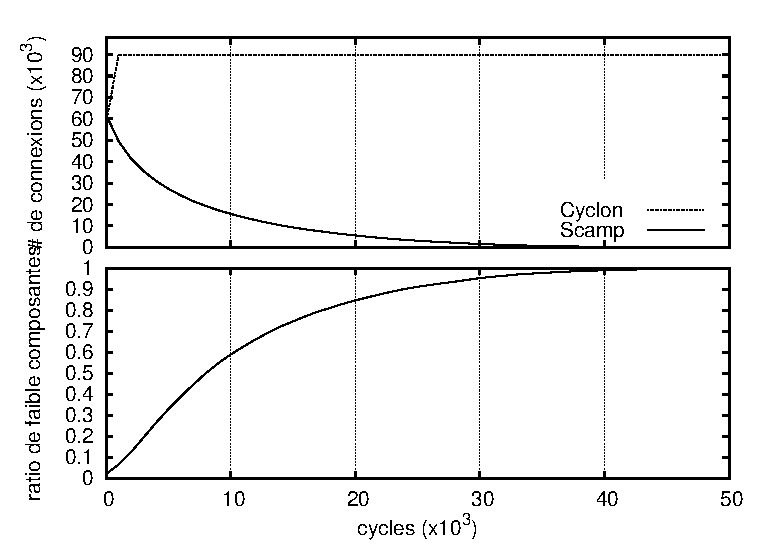
\includegraphics[width=0.65\textwidth]{img/network/motivation.eps}
  \end{center}

\end{frame}


\begin{frame}{Communication}{Définition du problème}

\begin{block}{Un protocole d'échantillonnage adaptatif}
  Soit $t$ une unité de temps arbitraire, soit $\mathcal{N}^t$ l'ensemble des
  membres non-byzantins du réseau à un instant $t$ et soit $P_i^t$ la vue
  partielle du nœud $n_i \in \mathcal{N}^t$. Un protocole d'échantillonnage
  aléatoire de pairs efficace doit assurer les propriétés suivantes :
  \begin{enumerate}
  \item Taille des vues partielles : \hfill $\forall n_i \in \mathcal{N}^t$,
    $|P_i^t| \approx \mathcal{O}(\ln |\mathcal{N}^t|)$
  \item Établissement de connexion : \hfill $\mathcal{O}(1)$
  \end{enumerate}
\end{block}

\begin{itemize}
\item [$\rightarrow$] Les vues partielles reflètent les besoins du réseau;
\item [$\rightarrow$] Limiter le nombre de sauts pour établir une connexion.
\end{itemize}

\end{frame}


\begin{frame}{Communication}{\SPRAY}

  \SPRAY :
  \begin{itemize}
  \item Protocole d'échantillonnage aléatoire de pairs;
    \vspace{0.25cm}
  \item Invariant : nombre de connexions
    $\approx |\mathcal{N}| \log |\mathcal{N}|$, sans connaissance globale, i.e.,
    $|\mathcal{N}|$ n'est connu de personne.
    \vspace{0.25cm}
  \item Établissement de connexions de proche en proche.
  \end{itemize}
    
  \vspace{1cm}

  Le réseau est \textbf{dynamique} : à n'importe quel moment, un pair peut
  rejoindre ou quitter le réseau. \\
  
  \vspace{1cm}

  \begin{minipage}{0.32\textwidth}
    \begin{center}
      \begin{tikzpicture}{scale=1}

  \newcommand\X{65pt};
  \newcommand\Y{15pt};


  \draw[->] (5+0*\X, 0*\Y) -- node[anchor=north]{\small{rejoint}} (-27+1*\X, 0*\Y);

  \draw[fill=white, very thick, draw=darkblue]
  (0*\X, 0*\Y) node{\DARKBLUE{$n$}} +(-5pt,-5pt) rectangle +(5pt,5pt);
  

  \draw[fill=white, dashed]
  (1*\X, 0*\Y) node{réseau $|\mathcal{N}|$} +(-27pt,-25pt) rectangle +(27pt,25pt);

 
\end{tikzpicture}
    \end{center}
  \end{minipage}
  \begin{minipage}{0.32\textwidth}
    \begin{center}
      \begin{tikzpicture}{scale=1}

  \newcommand\X{65pt};
  \newcommand\Y{15pt};


%  \draw[->] (0*\X, 0*\Y) -- node{rejoint} (-27+1*\X, 0*\Y);


  \draw[fill=white, dashed]
  (0*\X, 0*\Y) +(-27pt,-25pt) rectangle +(27pt,25pt);

  \draw[fill=white, very thick, draw=darkblue]
  (0*\X, 0*\Y) node{\DARKBLUE{$n$}} +(-5pt,-5pt) rectangle +(5pt,5pt);
  
  \draw[->] (  2+0*\X, -20+0*\Y ) to[out=15,in=-15] (2+0*\X, 20+0*\Y);
  \draw[<-] ( -2+0*\X, -20+0*\Y ) to[out=165,in=-165] (-2+0*\X, 20+0*\Y);

 
\end{tikzpicture}\\
    \end{center}
  \end{minipage}
  \begin{minipage}{0.32\textwidth}
    \begin{center}
      \begin{tikzpicture}{scale=1}

  \newcommand\X{65pt};
  \newcommand\Y{15pt};


  \draw[->] (27+0*\X, 0*\Y) -- node[anchor=north]{\small{quitte}} (-5+1*\X, 0*\Y);

  \draw[fill=white, very thick, draw=darkblue]
  (1*\X, 0*\Y) node{\DARKBLUE{$n$}} +(-5pt,-5pt) rectangle +(5pt,5pt);
  

  \draw[fill=white, dashed]
  (0*\X, 0*\Y) node{réseau $|\mathcal{N}|$} +(-27pt,-25pt) rectangle +(27pt,25pt);

 
\end{tikzpicture}
    \end{center}
  \end{minipage}

  \vspace{0.15cm}

  \begin{minipage}{0.32\textwidth}
    \begin{center}
      \small Ajoute $1+\log |\mathcal{N}|$ connexions
    \end{center}
  \end{minipage}
  \begin{minipage}{0.32\textwidth}
    \begin{center}
      % nothing
    \end{center}
  \end{minipage}
  \begin{minipage}{0.32\textwidth}
    \begin{center}
      \small Retire $1+\log |\mathcal{N}|$ connexions
    \end{center}
  \end{minipage}

\end{frame}


\begin{frame}{Communication}{Rejoindre le réseau}

  L'entrée d'un nouveau pair s'accompagne de $1+ \log {|\mathcal{N}|}$
  connexions.

  \vspace{0.5cm}
  
  \begin{itemize}
  \item \textbf{1 :} Le pair entrant se connecte à son contact;
  \item $\pmb{\log |\mathcal{N}|}$: On suppose que le protocole répond au
    problème et chaque pair possède une taille de vue partielle
    $\approx \log |\mathcal{N}|$.
  \end{itemize}

  \vspace{1cm}

  \begin{minipage}{0.32\textwidth}
    \begin{center}
      
\begin{tikzpicture}[scale=1.1]

  \newcommand\X{35pt};
  \newcommand\Y{15pt};

%  \draw(-0.75*\X, 0pt); %% positioning
%  \draw( 2.75*\X, 0pt); %% positioning

  \scriptsize
  \draw[->,dashed,very thick, color=darkblue](5+0*\X, 0*\Y) -- 
  node[anchor=south]{(a)}(-5+ 2*\X, 0*\Y);
  \draw[->] (-5+2*\X, 5pt) -- (5+\X, \Y);
  \draw[->] (-5+2*\X, 5pt) --  (5+\X, 2*\Y);
  \draw[->] (-5+2*\X, -5pt) -- (5+\X, -\Y);
  \draw[->] (-5+2*\X, -5pt) -- (5+\X, -2*\Y);

  \normalsize
  \draw[fill=white, very thick, draw=darkblue]
  (0*\X, 0*\Y) node{\DARKBLUE{$n_1$}} +(-5pt,-5pt) rectangle +(5pt,5pt);
  \draw[fill=white, very thick]
  (2*\X, 0*\Y) node{$n_2$} +(-5pt,-5pt) rectangle +(5pt,5pt);

  \draw[fill=white](1*\X,2*\Y) node{$n_6$} +(-5pt,-5pt) rectangle +(5pt,5pt);
  \draw[fill=white](1*\X,1*\Y) node{$n_5$} +(-5pt,-5pt) rectangle +(5pt,5pt);
  \draw[fill=white](1*\X,-1*\Y) node{$n_4$} +(-5pt,-5pt) rectangle +(5pt,5pt);
  \draw[fill=white](1*\X,-2*\Y) node{$n_3$} +(-5pt,-5pt) rectangle +(5pt,5pt);
  
\end{tikzpicture}
    \end{center}
  \end{minipage}
  \begin{minipage}{0.32\textwidth}
    \begin{center}
      
\begin{tikzpicture}[scale=1.1]

  \newcommand\X{35pt};
  \newcommand\Y{15pt};

%  \draw(-0.75*\X, 0pt); %% positioning
%  \draw( 2.75*\X, 0pt); %% positioning

  \scriptsize
  \draw[->](5+0*\X, 0*\Y) -- (-5+ 2*\X, 0*\Y);
  \draw[->, very thick, color=darkblue] (-5+2*\X, 5pt) -- (5+\X, \Y);
  \draw[->, very thick, color=darkblue] (-5+2*\X, 5pt) --
  node[anchor=south west]{(b)} (5+\X, 2*\Y);
  \draw[->, very thick, color=darkblue] (-5+2*\X, -5pt) -- (5+\X, -\Y);
  \draw[->, very thick, color=darkblue] (-5+2*\X, -5pt) --
  node[anchor=north west]{(b)}(5+\X, -2*\Y);

  \normalsize
  \draw[fill=white]
  (0*\X, 0*\Y) node{$n_1$} +(-5pt,-5pt) rectangle +(5pt,5pt);
  \draw[fill=white, very thick, draw=darkblue]
  (2*\X, 0*\Y) node{\DARKBLUE{$n_2$}} +(-5pt,-5pt) rectangle +(5pt,5pt);

  \draw[fill=white, very thick]
  (1*\X,2*\Y) node{$n_6$} +(-5pt,-5pt) rectangle +(5pt,5pt);
  \draw[fill=white, very thick]
  (1*\X,1*\Y) node{$n_5$} +(-5pt,-5pt) rectangle +(5pt,5pt);
  \draw[fill=white, very thick]
  (1*\X,-1*\Y) node{$n_4$} +(-5pt,-5pt) rectangle +(5pt,5pt);
  \draw[fill=white, very thick]
  (1*\X,-2*\Y) node{$n_3$} +(-5pt,-5pt) rectangle +(5pt,5pt);

\end{tikzpicture}
    \end{center}
  \end{minipage}
  \begin{minipage}{0.32\textwidth}
    \begin{center}
      
\begin{tikzpicture}[scale=1.1]

  \newcommand\X{35pt};
  \newcommand\Y{15pt};

%  \draw(-0.75*\X, 0pt); %% positioning
%  \draw( 2.75*\X, 0pt); %% positioning

  \scriptsize
  \draw[->](5+0*\X, 0*\Y) -- (-5+ 2*\X, 0*\Y);
  \draw[->] (-5+2*\X, 5pt) -- (5+\X, \Y);
  \draw[->] (-5+2*\X, 5pt) -- (5+\X, 2*\Y);
  \draw[->] (-5+2*\X, -5pt) -- (5+\X, -\Y);
  \draw[->] (-5+2*\X, -5pt) -- (5+\X, -2*\Y);

  \draw[->,dashed, very thick, color=darkblue](-5+\X, 2*\Y) --
  node[anchor=south east]{(c)} ( 5pt,5pt);
  \draw[->,dashed, very thick, color=darkblue](-5+\X, 1*\Y) -- ( 5pt,5pt);
  \draw[->,dashed, very thick, color=darkblue](-5+\X, -1*\Y) -- ( 5pt,-5pt);
  \draw[->,dashed, very thick, color=darkblue](-5+\X, -2*\Y) --
  node[anchor=north east]{(c)}( 5pt,-5pt);

  \normalsize
  \draw[fill=white, very thick]
  (0*\X, 0*\Y) node{$n_1$} +(-5pt,-5pt) rectangle +(5pt,5pt);
  \draw[fill=white]
  (2*\X, 0*\Y) node{$n_2$} +(-5pt,-5pt) rectangle +(5pt,5pt);

  \draw[fill=white, very thick, draw=darkblue]
  (1*\X,2*\Y) node{\DARKBLUE{$n_6$}} +(-5pt,-5pt) rectangle +(5pt,5pt);
  \draw[fill=white, very thick, draw=darkblue]
  (1*\X,1*\Y) node{\DARKBLUE{$n_5$}} +(-5pt,-5pt) rectangle +(5pt,5pt);
  \draw[fill=white, very thick, draw=darkblue]
  (1*\X,-1*\Y) node{\DARKBLUE{$n_4$}} +(-5pt,-5pt) rectangle +(5pt,5pt);
  \draw[fill=white, very thick, draw=darkblue]
  (1*\X,-2*\Y) node{\DARKBLUE{$n_3$}} +(-5pt,-5pt) rectangle +(5pt,5pt);
 

\end{tikzpicture}
    \end{center}
  \end{minipage}

  \vspace{1cm}
  
  \large
  \begin{itemize}
  \item [$\Rightarrow$] \textbf{Les vues partielles sont déséquilibrées}
  \end{itemize}

\end{frame}


\begin{frame}{Communication}{Échanges périodiques}
 
  Le nombre de connexions reste \textbf{constant}.
 
  \vspace{0.5cm}

  Les deux pairs impliqués dans l'échange périodique donne la \textbf{moitié} de
  leur vue partielle. Les pairs sont choisis \textbf{aléatoirement}.
  \begin{itemize}
  \item [$\rightarrow$] La taille des vues converge vers la \textbf{moyenne} des
    deux.
  \end{itemize}
  

  \vspace{0.5cm}\hspace{-1cm}
  \begin{minipage}{0.32\textwidth}
    \begin{center}
      
\begin{tikzpicture}[scale=1]

  \newcommand\X{35pt};
  \newcommand\Y{15pt};

  \draw[->](5+0*\X, 0*\Y) -- (-5+ 2*\X, 0*\Y); %% 1 -> 2
  \draw[->] (-5+2*\X, 5pt) -- (5+\X, \Y);
  \draw[->](2*\X,5pt) -- (5+1*\X, 2*\Y); %% 2 -> 6
  \draw[->] (-5+2*\X, -5pt) -- (5+\X, -\Y);
  \draw[->] (-5+2*\X, -5pt) -- (5+\X, -2*\Y);

  \draw[->,very thick, color=darkblue](-5+\X,2*\Y) -- (0pt,5pt); %% 6 -> 1

  \draw[->](-5+\X, 1*\Y) -- ( 5pt,5pt);
  \draw[->](-5+\X, -1*\Y) -- ( 5pt,-5pt);
  \draw[->](-5+\X, -2*\Y) -- ( 5pt,-5pt);

  \draw[->](-5+\X, 5+2*\Y)to[out=120,in=30](0pt,5+2*\Y); %% 6 -> 7
  \draw[->](-5+\X, 5+2*\Y)to[out=120,in=30](-5-\Y ,5+2*\Y); %% 6 -> 8
  \draw[->](-5+\X, 5+2*\Y)to[out=120,in=30](-10-2*\Y,5+2*\Y); %% 6 -> 9

  \normalsize
  \draw[fill=white, very thick]
  (0*\X, 0*\Y) node{$n_1$} +(-5pt,-5pt) rectangle +(5pt,5pt);
  \draw[fill=white](2*\X, 0*\Y) node{$n_2$} +(-5pt,-5pt) rectangle +(5pt,5pt);

  \draw[fill=white,very thick, draw=darkblue]
  (1*\X,2*\Y) node{\DARKBLUE{$n_6$}} +(-5pt,-5pt) rectangle +(5pt,5pt);
  \draw[fill=white](1*\X,1*\Y) node{$n_5$} +(-5pt,-5pt) rectangle +(5pt,5pt);
  \draw[fill=white](1*\X,-1*\Y) node{$n_4$} +(-5pt,-5pt) rectangle +(5pt,5pt);
  \draw[fill=white](1*\X,-2*\Y) node{$n_3$} +(-5pt,-5pt) rectangle +(5pt,5pt);

  \draw[fill=white]( 0*\X,2*\Y)
  node{$n_7$} +(-5pt,-5pt) rectangle +(5pt,5pt);
  \draw[fill=white](-5+-\Y,2*\Y)node{$n_8$} +(-5pt,-5pt) rectangle +(5pt,5pt);
  \draw[fill=white, draw=darkblue](-10+-2*\Y,2*\Y)
  node{\DARKBLUE{$n_9$}} +(-5pt,-5pt) rectangle +(5pt,5pt);
  

\end{tikzpicture}
    \end{center}
  \end{minipage}
  \hspace{0.35cm}
  \begin{minipage}{0.32\textwidth}
    \begin{center}
      
\begin{tikzpicture}[scale=1]

  \newcommand\X{35pt};
  \newcommand\Y{15pt};

  \draw[->](5+0*\X, 0*\Y) -- (-5+ 2*\X, 0*\Y); %% 1 -> 2
  \draw[->] (-5+2*\X, 5pt) -- (5+\X, \Y);
  \draw[->](2*\X,5pt) -- (5+1*\X, 2*\Y); %% 2 -> 6
  \draw[->] (-5+2*\X, -5pt) -- (5+\X, -\Y);
  \draw[->] (-5+2*\X, -5pt) -- (5+\X, -2*\Y);

  \draw[->,dashed, very thick, color=darkblue](0pt,5pt)--(-5+\X, 2*\Y); %% 1 -> 6

  \draw[->](-5+\X, 1*\Y) -- ( 5pt,5pt);
  \draw[->](-5+\X, -1*\Y) -- ( 5pt,-5pt);
  \draw[->](-5+\X, -2*\Y) -- ( 5pt,-5pt);

  \draw[->](-5+\X, 5+2*\Y)to[out=120,in=30](0pt,5+2*\Y); %% 6 -> 7
  \draw[->](-5+\X, 5+2*\Y)to[out=120,in=30](-5-\Y ,5+2*\Y); %% 6 -> 8
  
  \draw[->,dashed, very thick, color=darkblue](-5pt,5pt)--(-10-2*\Y,-5+2*\Y); %% 1 -> 9

  \normalsize
  \draw[fill=white, very thick]
  (0*\X, 0*\Y) node{$n_1$} +(-5pt,-5pt) rectangle +(5pt,5pt);
  \draw[fill=white, draw=darkblue](2*\X, 0*\Y)
  node{\DARKBLUE{$n_2$}} +(-5pt,-5pt) rectangle +(5pt,5pt);

  \draw[fill=white,very thick]
  (1*\X,2*\Y) node{$n_6$} +(-5pt,-5pt) rectangle +(5pt,5pt);
  \draw[fill=white](1*\X,1*\Y) node{$n_5$} +(-5pt,-5pt) rectangle +(5pt,5pt);
  \draw[fill=white](1*\X,-1*\Y) node{$n_4$} +(-5pt,-5pt) rectangle +(5pt,5pt);
  \draw[fill=white](1*\X,-2*\Y) node{$n_3$} +(-5pt,-5pt) rectangle +(5pt,5pt);

  \draw[fill=white]( 0*\X,2*\Y)
  node{$n_7$} +(-5pt,-5pt) rectangle +(5pt,5pt);
  \draw[fill=white](-5+-\Y,2*\Y)node{$n_8$} +(-5pt,-5pt) rectangle +(5pt,5pt);
  \draw[fill=white](-10+-2*\Y,2*\Y) node{$n_9$} +(-5pt,-5pt) rectangle +(5pt,5pt);
  

\end{tikzpicture}
    \end{center}
  \end{minipage}
  \hspace{0.35cm}
  \begin{minipage}{0.32\textwidth}
    \begin{center}
      
\begin{tikzpicture}[scale=1]

  \newcommand\X{35pt};
  \newcommand\Y{15pt};

  \draw[->] (-5+2*\X, 5pt) -- (5+\X, \Y);
  \draw[->,dashed, very thick, color=darkblue]
  (5+\X, 2*\Y)to[out=-20,in=110](2*\X, 5pt); %% 6 -> 2
  \draw[->](2*\X,5pt)to[out=160,in=-70](5+1*\X, 2*\Y); %% 2 -> 6
  \draw[->] (-5+2*\X, -5pt) -- (5+\X, -\Y);
  \draw[->] (-5+2*\X, -5pt) -- (5+\X, -2*\Y);

  \draw[->](0pt,5pt)--(-5+\X, 2*\Y); %% 1 -> 6

  \draw[->](-5+\X, 1*\Y) -- ( 5pt,5pt);
  \draw[->](-5+\X, -1*\Y) -- ( 5pt,-5pt);
  \draw[->](-5+\X, -2*\Y) -- ( 5pt,-5pt);

  \draw[->](-5+\X, 5+2*\Y)to[out=120,in=30](0pt,5+2*\Y); %% 6 -> 7
  \draw[->](-5+\X, 5+2*\Y)to[out=120,in=30](-5-\Y ,5+2*\Y); %% 6 -> 8
  
  \draw[->](-5pt,5pt)--(-10-2*\Y,-5+2*\Y); %% 1 -> 9

  \normalsize
  \draw[fill=white]
  (0*\X, 0*\Y) node{$n_1$} +(-5pt,-5pt) rectangle +(5pt,5pt);
  \draw[fill=white](2*\X, 0*\Y) node{$n_2$} +(-5pt,-5pt) rectangle +(5pt,5pt);

  \draw[fill=white,very thick]
  (1*\X,2*\Y) node{$n_6$} +(-5pt,-5pt) rectangle +(5pt,5pt);
  \draw[fill=white](1*\X,1*\Y) node{$n_5$} +(-5pt,-5pt) rectangle +(5pt,5pt);
  \draw[fill=white](1*\X,-1*\Y) node{$n_4$} +(-5pt,-5pt) rectangle +(5pt,5pt);
  \draw[fill=white](1*\X,-2*\Y) node{$n_3$} +(-5pt,-5pt) rectangle +(5pt,5pt);

  \draw[fill=white]( 0*\X,2*\Y)
  node{$n_7$} +(-5pt,-5pt) rectangle +(5pt,5pt);
  \draw[fill=white](-5+-\Y,2*\Y)node{$n_8$} +(-5pt,-5pt) rectangle +(5pt,5pt);
  \draw[fill=white](-10+-2*\Y,2*\Y) node{$n_9$} +(-5pt,-5pt) rectangle +(5pt,5pt);
  

\end{tikzpicture}
    \end{center}
  \end{minipage}

  \vspace{0.5cm}
  \large
  \begin{itemize}
  \item [$\Rightarrow$] \textbf{Équilibre rapidement la taille des vues
      partielles;}
  \item [$\Rightarrow$] \textbf{Disperse les groupes fortement connectés.}
  \end{itemize}
  
\end{frame}

\begin{frame}{Communication}{Quitter le réseau}

  Le départ d'un pair doit engendrer la suppression de $1+\log|\mathcal{N}|$ connexions.

  \vspace{0.5cm}

  Problème : la vue sortante + la vue entrante $\approx 2\log|\mathcal{N}|$
  \begin{itemize}
  \item $\pmb{\log|\mathcal{N}|}$ : La vue partielle du pair quittant le réseau;
  \item \textbf{1} : Un parmi les $\approx \log|\mathcal{N}|$ pairs détectant
    le départ ne recrée pas de connexion.
  \end{itemize}

  \vspace{0.5cm}\hspace{-1cm}
  \begin{minipage}{0.32\textwidth}
    \begin{center}
      
\begin{tikzpicture}[scale=0.9]

  \newcommand\X{35pt};
  \newcommand\Y{15pt};

  \large
  \draw[->](-5+\X, 1*\Y) --node{$\times$} ( 5pt,5pt);
  \draw[->](-5+\X, -1*\Y) --node{$\times$} ( 5pt,-5pt);
  \draw[->](-5+\X, -2*\Y) --node{$\times$} ( 5pt,-5pt);

  \draw[->, color=darkblue](-5pt,5pt)--
  node{\DARKBLUE{$\times$}}(-10-2*\Y,-5+2*\Y); %% 1 -> 9
  \draw[->, color=darkblue](-5pt,5pt)--
  node{\DARKBLUE{$\times$}}(-5-1*\Y,-5+2*\Y); %% 1 ->8 
  \draw[->, color=darkblue](-5pt,5pt)--
  node{\DARKBLUE{$\times$}}(0pt,-5+2*\Y); %% 1 -> 7
  \draw[->, color=darkblue](-5pt,5pt)--
  node{\DARKBLUE{$\times$}}(-5+\X,-5+2*\Y); %% 1 -> 6

  \normalsize
  \draw[->](5+ 1*\X, 5+ 1*\Y)--(-5+2*\X, 2*\Y); %% 5 -> 14
  \draw[->](5+1*\X,  1*\Y)--(-5+2*\X, 1*\Y); %% 5 -> 13 
  
  \draw[->](5+\X, 5-\Y) -- (-5+2*\X,0pt); %% 4 -> 12
  \draw[->](5+\X, -\Y) -- (-5+2*\X, -\Y); %% 4 -> 11
  
  \draw[->](5+\X, -2*\Y) -- (-5+2*\X, -2*\Y);
  
  \tiny
  \draw[fill=white,very thick, draw=darkblue]
  (0*\X, 0*\Y) node{\DARKBLUE{$n_1$}} +(-5pt,-5pt) rectangle +(5pt,5pt);
  \draw[thick, color=darkblue] (-5pt,-5pt) -- (5pt,5pt);
  \draw[thick, color=darkblue] (-5pt, 5pt) -- (5pt,-5pt);
  
  \draw[fill=white]
  (1*\X,1*\Y) node{$n_5$} +(-5pt,-5pt) rectangle +(5pt,5pt);
  \draw[fill=white]
  (1*\X,-1*\Y) node{$n_4$} +(-5pt,-5pt) rectangle +(5pt,5pt);
  \draw[fill=white]
  (1*\X,-2*\Y) node{$n_3$} +(-5pt,-5pt) rectangle +(5pt,5pt);

  \draw[fill=white](\X,2*\Y) node{$n_6$} +(-5pt,-5pt) rectangle +(5pt,5pt);

  \draw[fill=white]( 0*\X,2*\Y)
  node{$n_7$} +(-5pt,-5pt) rectangle +(5pt,5pt);
  \draw[fill=white](-5+-\Y,2*\Y)node{$n_8$} +(-5pt,-5pt) rectangle +(5pt,5pt);
  \draw[fill=white](-10+-2*\Y,2*\Y) node{$n_9$} +(-5pt,-5pt) rectangle +(5pt,5pt);
  
  \draw[fill=white](2*\X,2*\Y)node{$n_{14}$} +(-5pt,-5pt) rectangle +(5pt,5pt);
  \draw[fill=white](2*\X,1*\Y)node{$n_{13}$} +(-5pt,-5pt) rectangle +(5pt,5pt);
  \draw[fill=white](2*\X,0*\Y)node{$n_{12}$} +(-5pt,-5pt) rectangle +(5pt,5pt);
  \draw[fill=white](2*\X,-1*\Y)node{$n_{11}$}+(-5pt,-5pt) rectangle +(5pt,5pt);
  \draw[fill=white](2*\X,-2*\Y)node{$n_{10}$}+(-5pt,-5pt) rectangle +(5pt,5pt);

\end{tikzpicture}
    \end{center}
  \end{minipage}
  \hspace{0.45cm}
  \begin{minipage}{0.32\textwidth}
    \begin{center}
      
\begin{tikzpicture}[scale=0.9]

  \newcommand\X{35pt};
  \newcommand\Y{15pt};

  \large
  \draw[->, very thick, color=darkblue](-5+\X, 1*\Y) --
  node{\DARKBLUE{$\times$}} ( 5pt,5pt);
  \draw[->, very thick, color=darkblue](-5+\X, -1*\Y) --
  node{\DARKBLUE{$\times$}} ( 5pt,-5pt);
  \draw[->, very thick, color=darkblue](-5+\X, -2*\Y) --
  node{\DARKBLUE{$\times$}} ( 5pt,-5pt);

  \normalsize

  \draw[->](5+ 1*\X, 5+ 1*\Y)--(-5+2*\X, 2*\Y); %% 5 -> 14
  \draw[->](  5+1*\X, 1*\Y)--(-5+2*\X, 1*\Y); %% 5 -> 13 (v)
  
  \draw[->](5+\X, 5-\Y) -- (-5+2*\X,0pt); %% 4 -> 12
  \draw[->](5+\X, -\Y) -- (-5+2*\X, -\Y); %% 4 -> 11
  
  \draw[->](5+\X, -2*\Y) -- (-5+2*\X, -2*\Y);
  
  \tiny
  \draw[fill=white]
  (0*\X, 0*\Y) node{$n_1$} +(-5pt,-5pt) rectangle +(5pt,5pt);
  \draw (-5pt,-5pt) -- (5pt,5pt);
  \draw (-5pt, 5pt) -- (5pt,-5pt);
  
  \draw[fill=white, very thick, draw=darkblue]
  (1*\X,1*\Y) node{\DARKBLUE{$n_5$}} +(-5pt,-5pt) rectangle +(5pt,5pt);
  \draw[fill=white, very thick, draw=darkblue]
  (1*\X,-1*\Y) node{\DARKBLUE{$n_4$}} +(-5pt,-5pt) rectangle +(5pt,5pt);
  \draw[fill=white, very thick, draw=darkblue]
  (1*\X,-2*\Y) node{\DARKBLUE{$n_3$}} +(-5pt,-5pt) rectangle +(5pt,5pt);

  \draw[fill=white](\X,2*\Y) node{$n_6$} +(-5pt,-5pt) rectangle +(5pt,5pt);

  \draw[fill=white]( 0*\X,2*\Y)
  node{$n_7$} +(-5pt,-5pt) rectangle +(5pt,5pt);
  \draw[fill=white](-5+-\Y,2*\Y)node{$n_8$} +(-5pt,-5pt) rectangle +(5pt,5pt);
  \draw[fill=white](-10+-2*\Y,2*\Y) node{$n_9$} +(-5pt,-5pt) rectangle +(5pt,5pt);
  
  \draw[fill=white](2*\X,2*\Y)node{$n_{14}$} +(-5pt,-5pt) rectangle +(5pt,5pt);
  \draw[fill=white](2*\X,1*\Y)node{$n_{13}$} +(-5pt,-5pt) rectangle +(5pt,5pt);
  \draw[fill=white](2*\X,0*\Y)node{$n_{12}$} +(-5pt,-5pt) rectangle +(5pt,5pt);
  \draw[fill=white](2*\X,-1*\Y)node{$n_{11}$}+(-5pt,-5pt) rectangle +(5pt,5pt);
  \draw[fill=white](2*\X,-2*\Y)node{$n_{10}$}+(-5pt,-5pt) rectangle +(5pt,5pt);

\end{tikzpicture}
    \end{center}
  \end{minipage}
  \hspace{0.45cm}
  \begin{minipage}{0.32\textwidth}
    \begin{center}
      
\begin{tikzpicture}[scale=0.9]

  \newcommand\X{35pt};
  \newcommand\Y{15pt};

  \draw[->](5+ 1*\X, 5+ 1*\Y)--(-5+2*\X, 2*\Y); %% 5 -> 14
  \draw[->](5+1*\X, 2.5+ 1*\Y)--(-5+2*\X, 2.5+ 1*\Y); %% 5 -> 13 (^)
  \draw[->,dashed, very thick, color=darkblue]
  (  5+1*\X,-2.5+1*\Y)--(-5+2*\X,-2.5+1*\Y); %% 5 -> 13 (v)
  
  \draw[->](5+\X, 5-\Y) -- (-5+2*\X,0pt); %% 4 -> 12
  \draw[->](5+\X, -\Y) -- (-5+2*\X, -\Y); %% 4 -> 11
  
  \draw[->](5+\X, 2.5-2*\Y) -- (-5+2*\X, 2.5-2*\Y);
  \draw[->,dashed, very thick, color=darkblue](5+\X, -2.5-2*\Y) -- (-5+2*\X , -2.5-2*\Y);
  
  \tiny
  \draw[fill=white]
  (0*\X, 0*\Y) node{$n_1$} +(-5pt,-5pt) rectangle +(5pt,5pt);
  \draw (-5pt,-5pt) -- (5pt,5pt);
  \draw (-5pt, 5pt) -- (5pt,-5pt);
  
  \draw[fill=white, very thick]
  (1*\X,1*\Y) node{$n_5$} +(-5pt,-5pt) rectangle +(5pt,5pt);
  \draw[fill=white, very thick]
  (1*\X,-1*\Y) node{$n_4$} +(-5pt,-5pt) rectangle +(5pt,5pt);
  \draw[fill=white, very thick]
  (1*\X,-2*\Y) node{$n_3$} +(-5pt,-5pt) rectangle +(5pt,5pt);

  \draw[fill=white](\X,2*\Y) node{$n_6$} +(-5pt,-5pt) rectangle +(5pt,5pt);

  \draw[fill=white]( 0*\X,2*\Y)
  node{$n_7$} +(-5pt,-5pt) rectangle +(5pt,5pt);
  \draw[fill=white](-5+-\Y,2*\Y)node{$n_8$} +(-5pt,-5pt) rectangle +(5pt,5pt);
  \draw[fill=white](-10+-2*\Y,2*\Y) node{$n_9$} +(-5pt,-5pt) rectangle +(5pt,5pt);
  
  \draw[fill=white](2*\X,2*\Y)node{$n_{14}$} +(-5pt,-5pt) rectangle +(5pt,5pt);
  \draw[fill=white](2*\X,1*\Y)node{$n_{13}$} +(-5pt,-5pt) rectangle +(5pt,5pt);
  \draw[fill=white](2*\X,0*\Y)node{$n_{12}$} +(-5pt,-5pt) rectangle +(5pt,5pt);
  \draw[fill=white](2*\X,-1*\Y)node{$n_{11}$}+(-5pt,-5pt) rectangle +(5pt,5pt);
  \draw[fill=white](2*\X,-2*\Y)node{$n_{10}$}+(-5pt,-5pt) rectangle +(5pt,5pt);

\end{tikzpicture}
    \end{center}
  \end{minipage}

  \vspace{1cm}
  \large
  \begin{itemize}
  \item [$\Rightarrow$] \textbf{Présence de doublons assure la cohérence du
      nombre de connexions.}
  \end{itemize}
 
\end{frame}


\begin{frame}{Communication}{Expérimentations}

  Simulations \PEERSIM.
  
  \vspace{0.5cm}

  Résultats attendus :
  \begin{itemize}
  \item Convergence rapide vers un réseau possédant des propriétés similaires à
    celles des graphes aléatoires;
  \item Les doublons sont peu nombreux et n'impactent pas significativement les
    propriétés du réseau;
  \item Les protocoles basés sur \SPRAY bénéficient de son adaptativité.
  \end{itemize}

\end{frame}


\begin{frame}{Communication}{Problème d'établissement de connexions}

  \begin{center}
    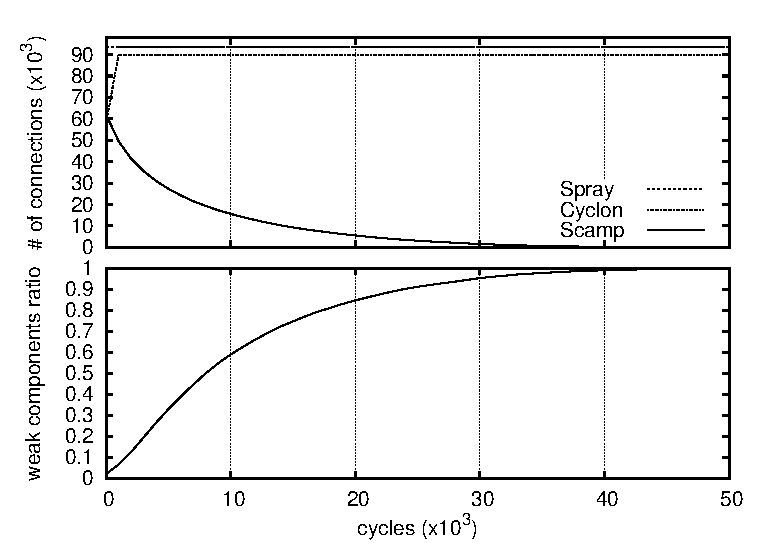
\includegraphics[width=1\textwidth]{img/network/degen.eps}
  \end{center}

\end{frame}


\begin{frame}{Communication}{Les vues partielles s'adaptent}

  \begin{center}
    \begin{tikzpicture}
    \draw(0pt,0pt) node{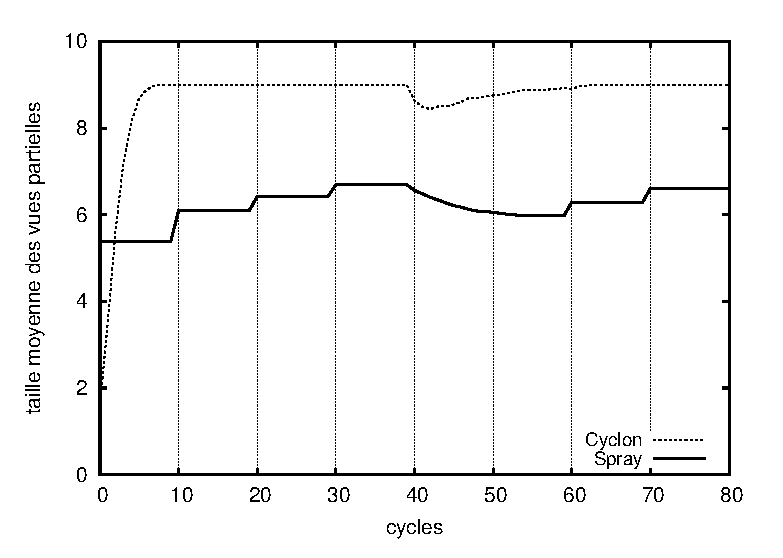
\includegraphics[width=1\textwidth]{img/network/avgpv.eps}};
    \draw(-130pt, 0pt) node{$250$};
    \draw(-95pt,  0pt) node{$+250$};
    \draw(-60pt,  0pt) node{$+250$};
    \draw(-30pt,  0pt) node{$+250$};
    \draw( 2pt,   0pt) node{$-500$};
    \draw( 70pt,  0pt) node{$+250$};
    \draw( 105pt, 0pt) node{$+250$};
    
    \end{tikzpicture}
  \end{center}
\end{frame}


\begin{frame}{Communication}{Coefficient d'agglomération diminue rapidement}
  \hspace{-1cm}
  \begin{minipage}{0.47\textwidth}
    \begin{center}
      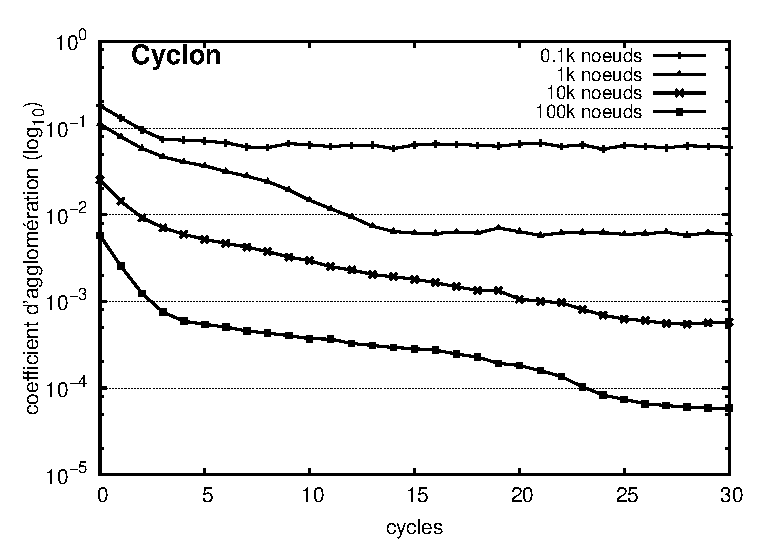
\includegraphics[width=1.23\textwidth]{img/network/cycloncluster.eps}
    \end{center}
  \end{minipage}
  \hfill
  \begin{minipage}{0.47\textwidth}
      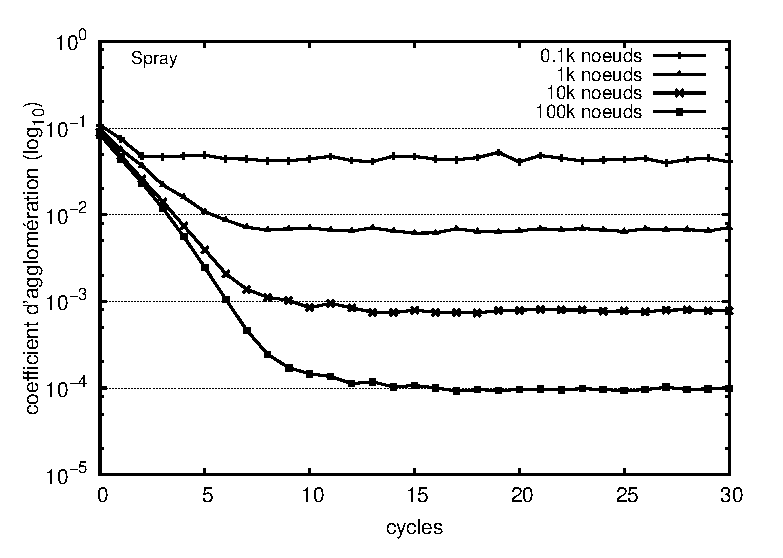
\includegraphics[width=1.23\textwidth]{img/network/spraycluster.eps}
  \end{minipage}

  \vspace{0.5cm}

  \begin{itemize}
  \item \CYCLON configuré avec
    \begin{itemize}
    \item  $\ln(1000) \approx 7$ voisins et
    \item mélange de $3$ voisins.
    \end{itemize}
  \end{itemize}

\end{frame}


\begin{frame}{Communication}{Faible taux de doublons}
  \begin{center}
    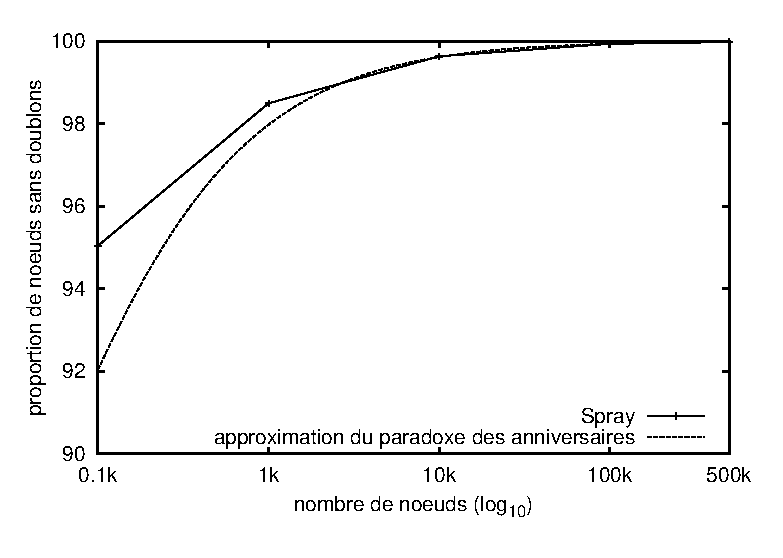
\includegraphics[width=1\textwidth]{img/network/duplicates.eps}
  \end{center}
\end{frame}


\begin{frame}{Communication}{Cas de la diffusion de messages}

  \begin{center}
    

\begin{tikzpicture}

  \newcommand\X{100pt};
  \newcommand\Y{-60pt};


  \draw[fill=white](0*\X,0*\Y) node{$n$} +(-5pt,-5pt) rectangle +(5pt,5pt);

  \foreach \y in {0,...,30}
  {
    \draw[->](5+0*\X, 0*\Y) -- (-5+1*\X, {(4*\y)+\Y});
  }
  

  \only<2->{
    \foreach \y in { -2*4, -14*4, 10*4, 3*4, -12*4, 8*4}
    {
      \draw[->, very thick, color=darkblue](5+0*\X, 0*\Y) -- (-5+1*\X, \y pt);
    }
  }

  \only<3->{
    \foreach \y in { -12*4, -3*4, 11*4, 0*4, -9*4, -5*4}
    {
      \draw[->, very thick, color=termithgreen](5+0*\X, 0*\Y) -- (-5+1*\X, \y pt);
    }
  }
    
  \only<4->{
    \foreach \y in { -8*4, -15*4, 2*4, 3*4, 8*4, 15*4}
    {
      \draw[->, very thick, color=termithorange](5+0*\X, 0*\Y) -- (-5+1*\X, \y pt);
    }    
  }

\end{tikzpicture}
  \end{center}
  
  \begin{center}
    \uncover<2->{\DARKBLUE{diffuse($msg_1$)}} \uncover<3->{\textcolor{termithgreen}{diffuse($msg_2$)}} \uncover<4->{\textcolor{termithorange}{$diffuse(msg_3)$}}
  \end{center}

  \begin{itemize}
  \item \CYCLON 
    \begin{enumerate}
    \item vue partielle de 30 voisins, fanout de $\ln(100)+1\approx 6$;
    \item vue partielle de 30 voisins, fanout de  $\ln(100)+3 \approx 8$.
    \end{enumerate}
  \item \SPRAY
    \begin{enumerate}
    \item vue partielle de $6\cdot\ln|\mathcal{N}|$ voisins,
      fanout de $\ln(|\mathcal{N}|)+1$;
    \item vue partielle de $6\cdot\ln|\mathcal{N}|$ voisins,
      fanout de $\ln(|\mathcal{N}|)+3$;
    \end{enumerate}
  \end{itemize}

\end{frame}


\begin{frame}{Communication}{Le taux d'erreur reste constant}
  \begin{center}
    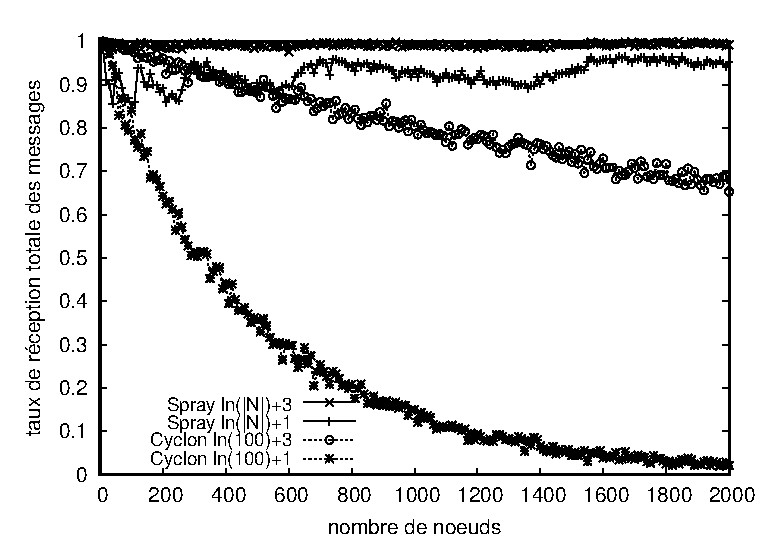
\includegraphics[width=1\textwidth]{img/network/hardrate.eps}
  \end{center} 
\end{frame}


\begin{frame}{Communication}{Le pic de popularité est mieux géré}
  \begin{center}
    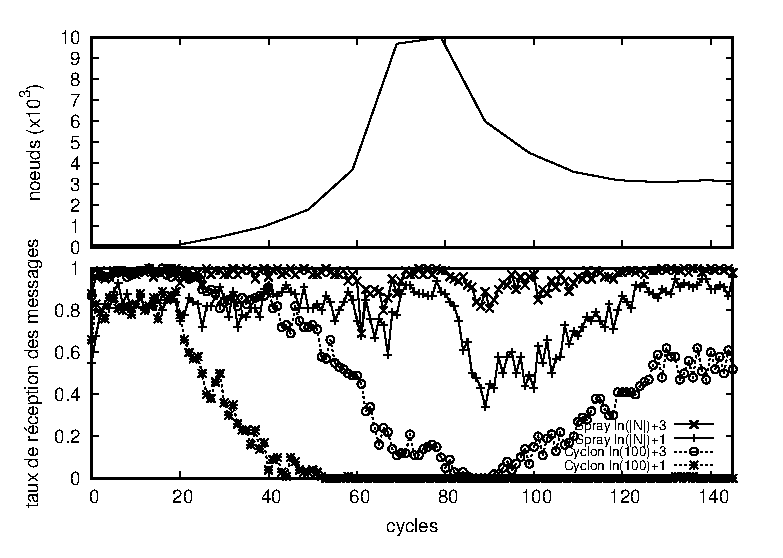
\includegraphics[width=1\textwidth]{img/network/peak.eps}
  \end{center} 
\end{frame}


\begin{frame}{Communication}{Conclusion}
  
  \begin{itemize}
  \item \SPRAY est un protocole d'échantillonnage aléatoire de pair adaptatif.
  \item \SPRAY est adapté au processus complexe d'établissement de connexion de
    WebRTC.
  \end{itemize}

  \vspace{1cm}

  \begin{itemize}
  \item Les protocoles construits au dessus de \SPRAY bénéficient de cette
    adaptativité.
  \end{itemize}

\end{frame}

\begin{frame}{Communication}{Perspective}

  \begin{block}{Les réseaux fusionnant préservent leurs propriétés}
    Soit $\mathcal{N}_1,\, \mathcal{N}_2,\, \ldots ,\, \mathcal{N}_k$ des réseaux
    de taille arbitraire. On a : \vspace{-5pt}
    \begin{equation}
      \sum\limits_{i = 1}^k |\mathcal{N}_i|\ln (|\mathcal{N}_i|) < (\sum\limits_{i = 1}^k |\mathcal{N}_i|)\ln{(\sum\limits_{i=1}^k |\mathcal{N}_i|)}
    \end{equation}
    Comment adapter le nombre d'arcs effectifs (à gauche) pour qu'il atteigne le
    nombre d'arcs requis (à droite)?
  \end{block}

  \begin{minipage}{0.325\textwidth}
    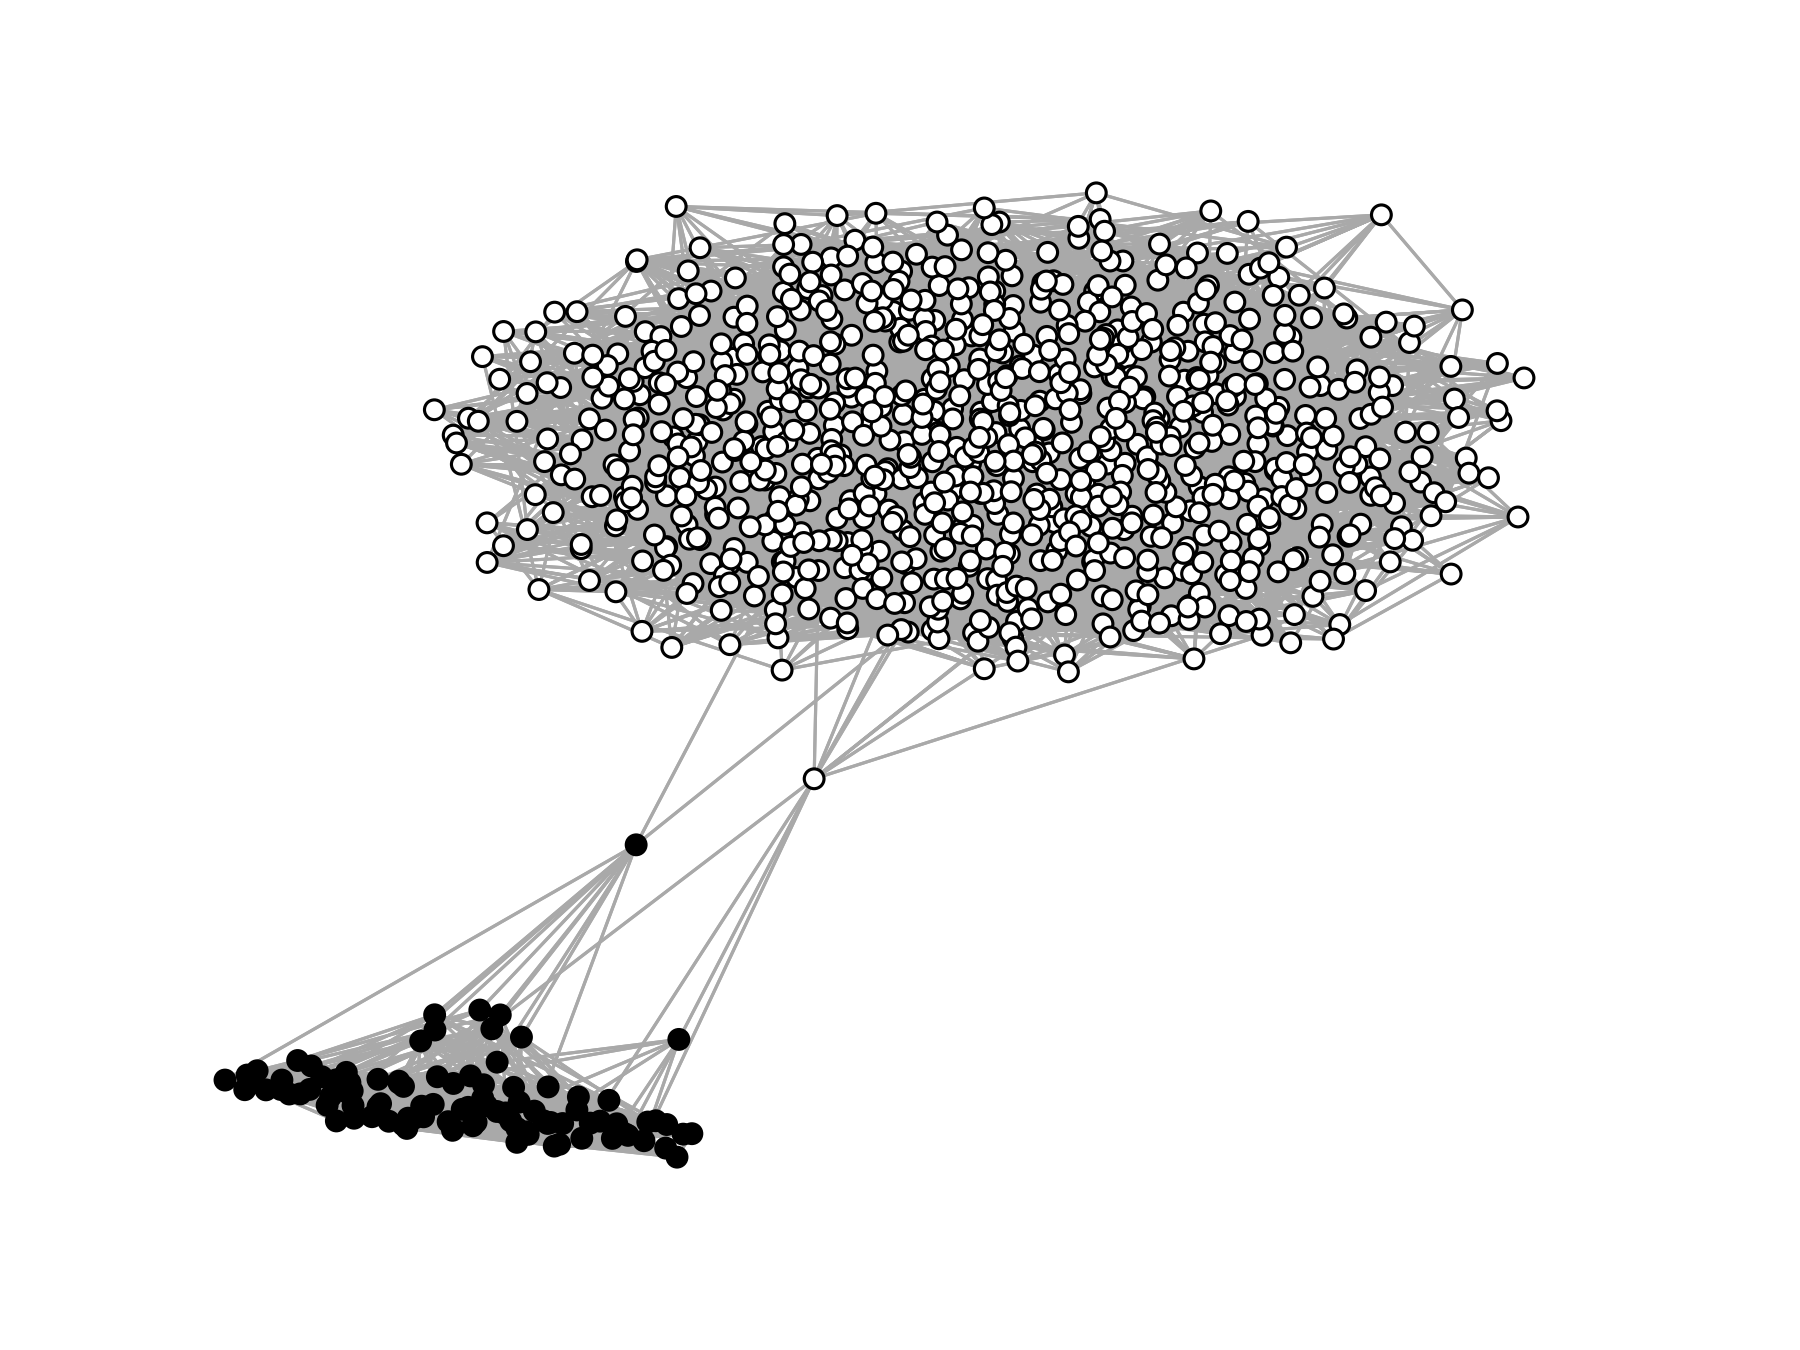
\includegraphics[width=1.2\textwidth]{img/graphA.png}
  \end{minipage}
  \begin{minipage}{0.325\textwidth}
    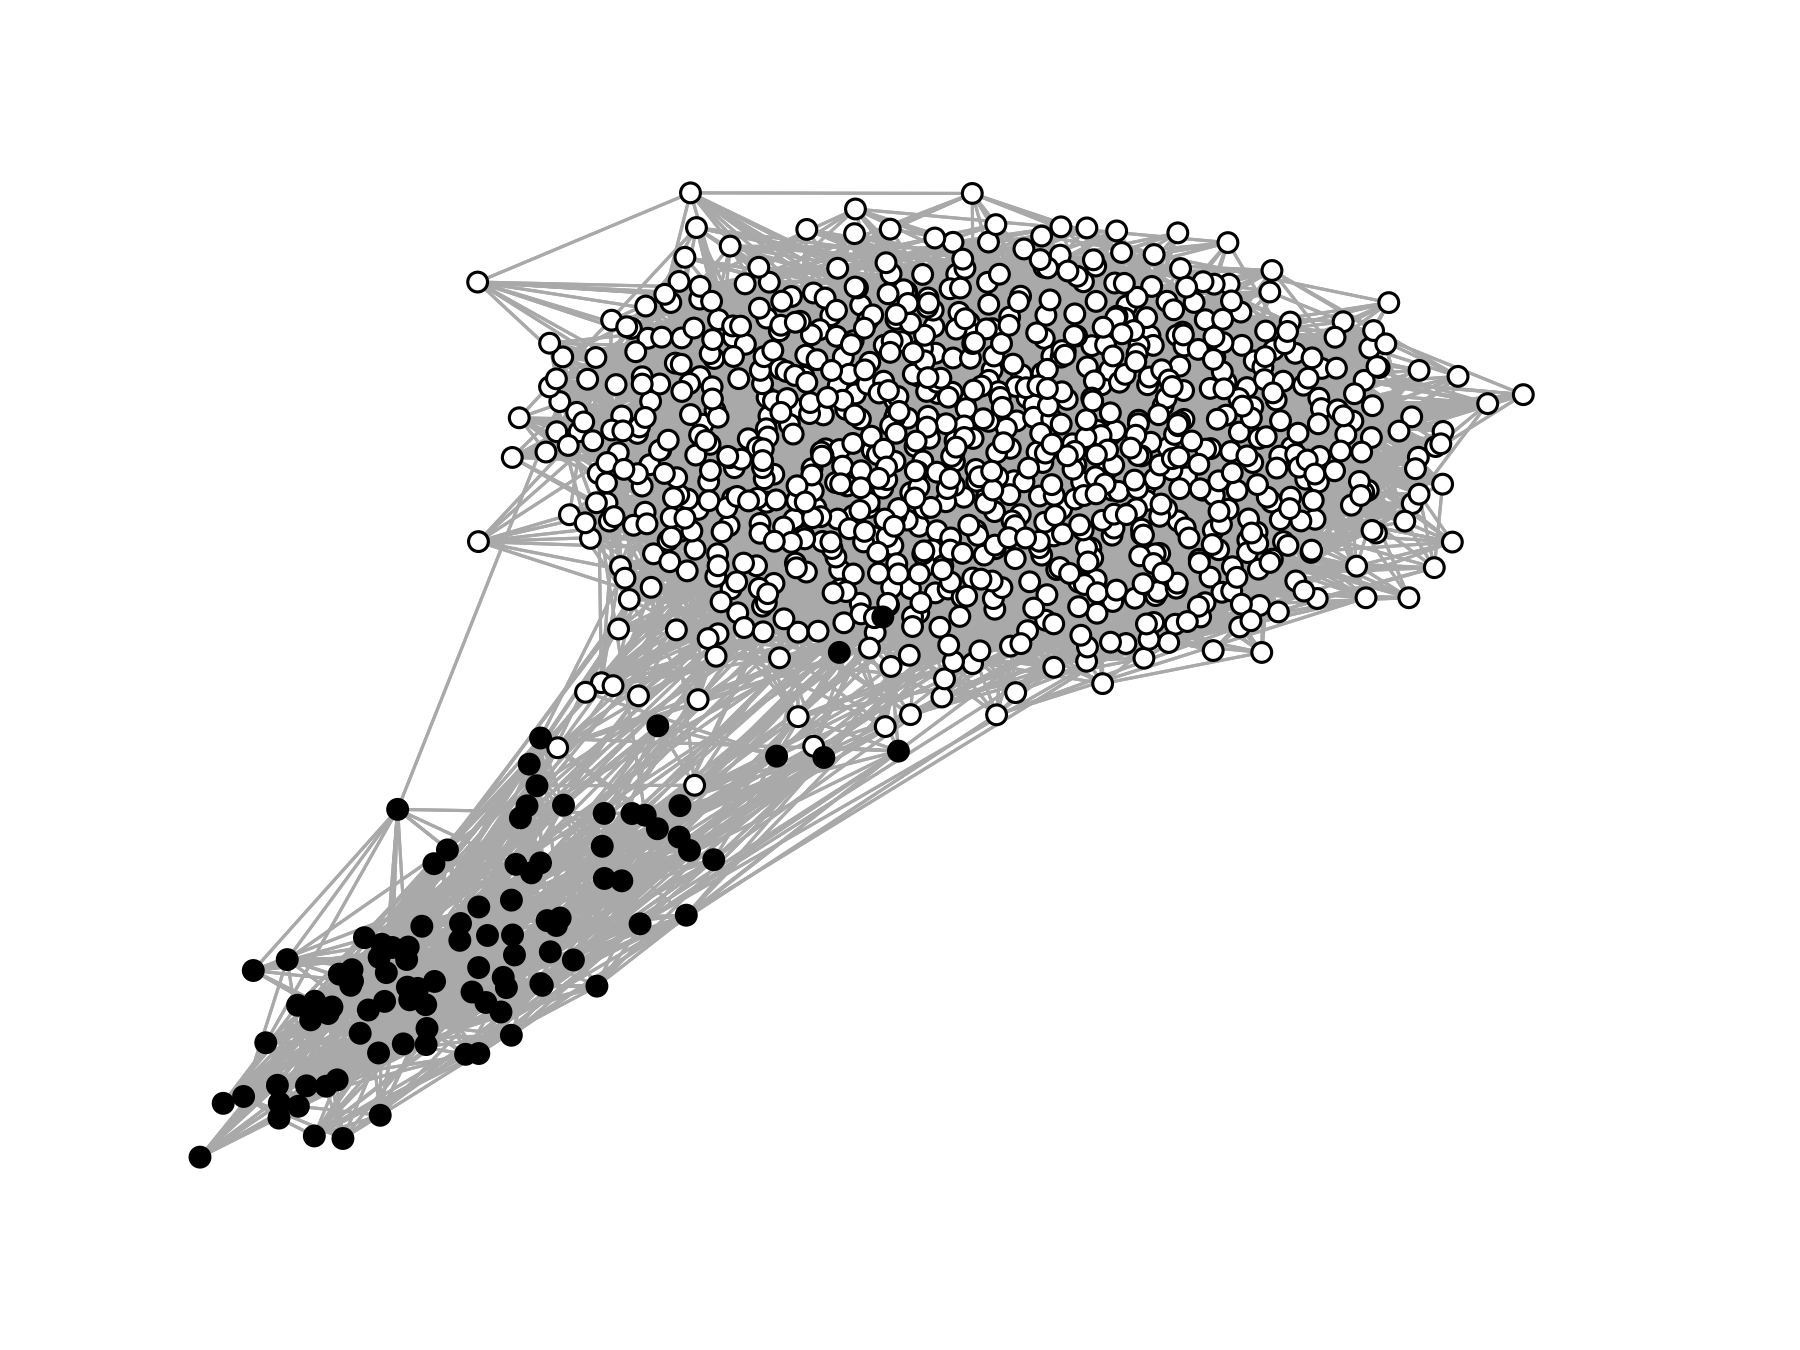
\includegraphics[width=1.2\textwidth]{img/graphB.png}
  \end{minipage}
  \begin{minipage}{0.325\textwidth}
    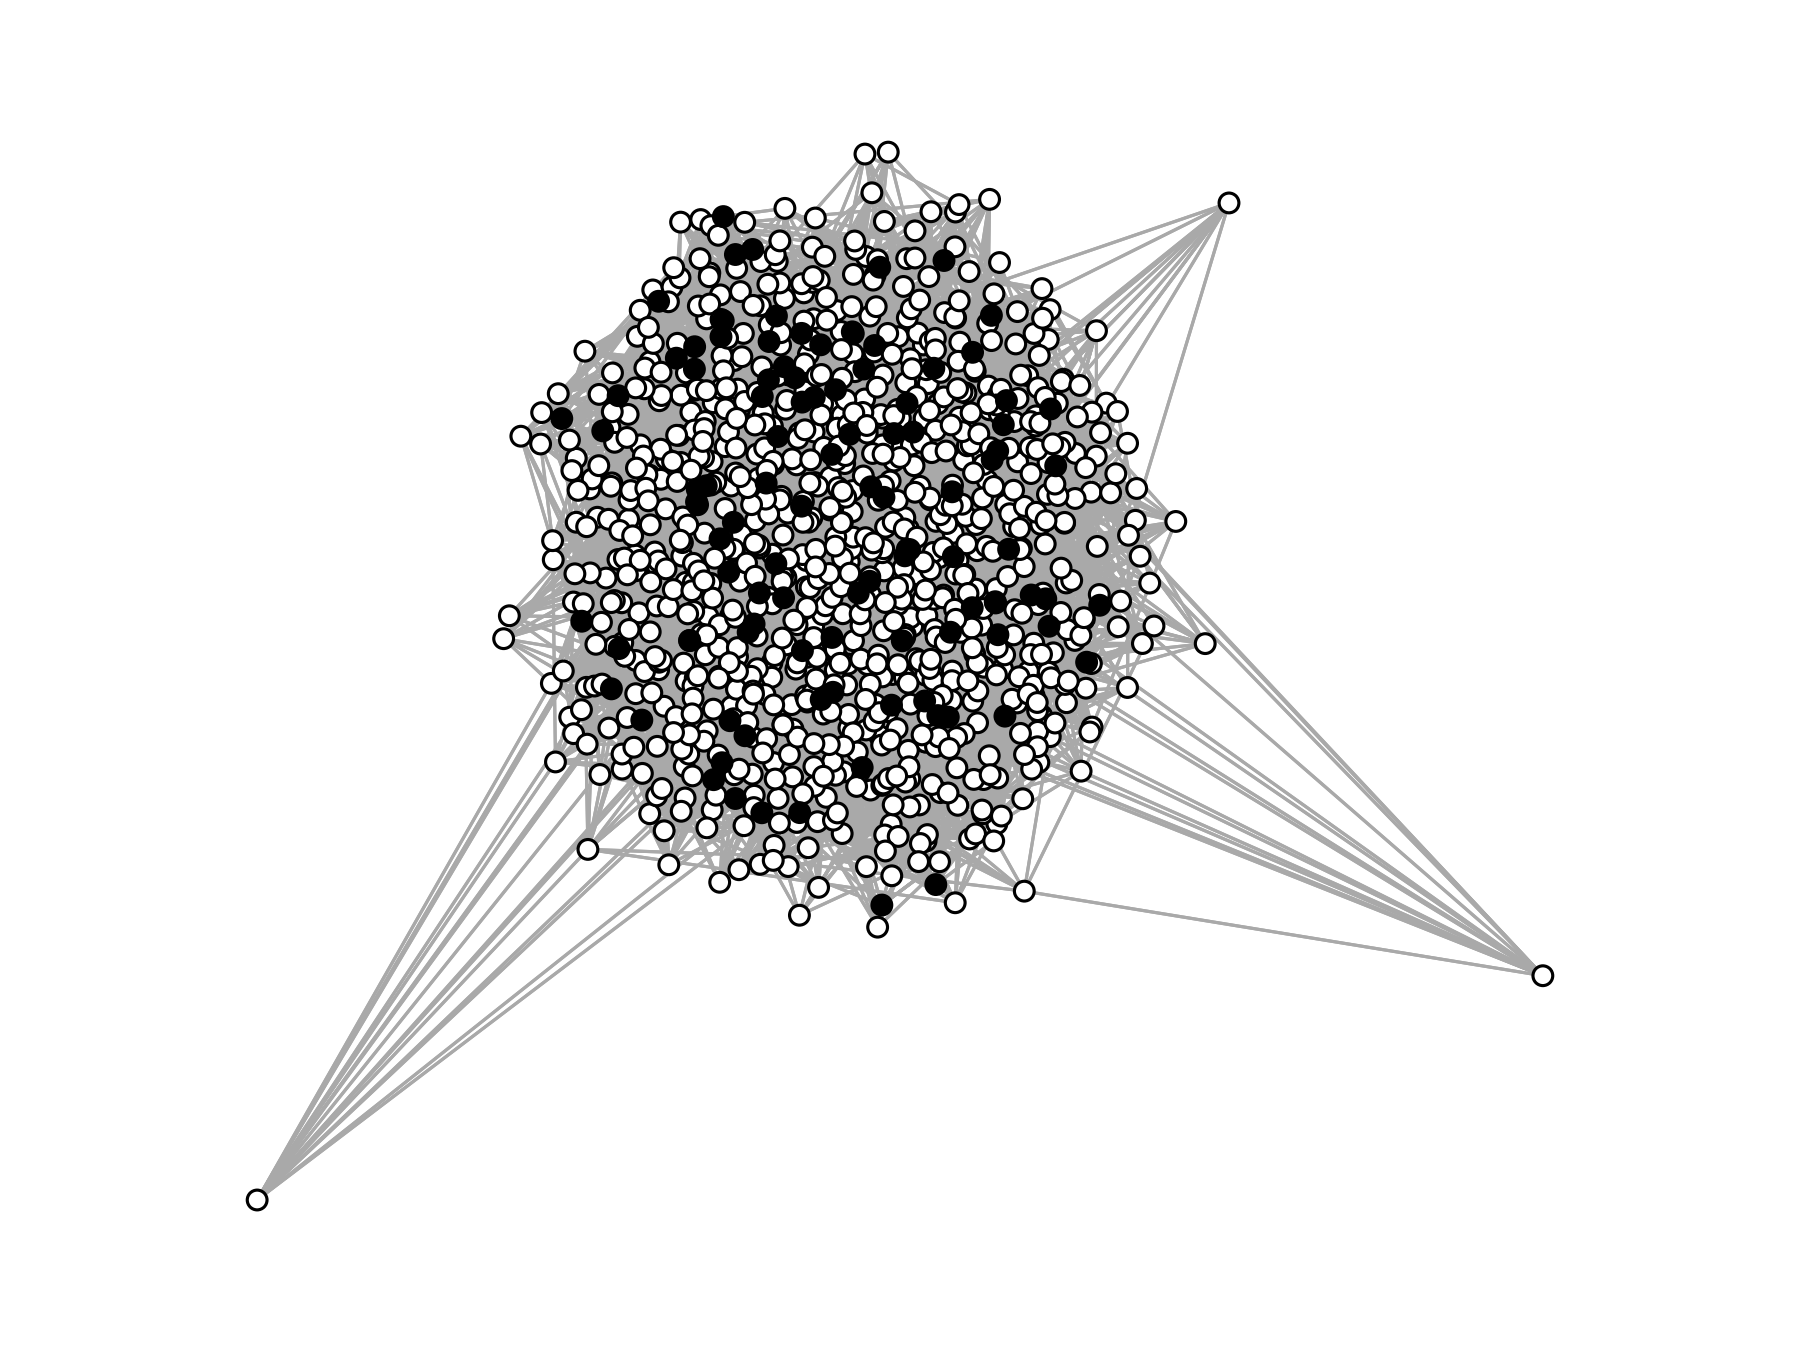
\includegraphics[width=1.2\textwidth]{img/graphC.png}
  \end{minipage}

\end{frame}


\begin{frame}{Communication}{Vues partielles adaptatives}

  \hspace{-1cm}
  \begin{minipage}{0.55\textwidth}
    \begin{itemize}
      \item \textbf{Chaque éditeur possède une copie locale du document;}
      \item \textbf{Chaque éditeur est connecté à d'autres éditeurs.}
      \vspace{0.5cm}
    \item Chaque caractère tapé est directement inséré dans la copie locale;
    \item La modification est disséminée à l'ensemble du réseau;
    \item Les éditeurs recevant la modification l'appliquent.
    \end{itemize}
  \end{minipage}
  \hfill
  \begin{minipage}{0.44\textwidth}
    \begin{center}
      
\begin{tikzpicture}[scale=1.3]

  \newcommand\X{35pt}
  \newcommand\Y{-35pt}
  
%  \small

%  \draw (-35-2*\X, 30pt);

  
%  \draw[fill=white] (-2*\X, 1.5*\Y) 
%  node{
\includegraphics[width=12pt]{img/crateicon.png}};
  % node{$e_9$}; % +(-5pt,-5pt) rectangle +(5pt,5pt);
  % \only<3>{
  %   \draw[<->, densely dashed, color=darkblue, very thick]
  %   (-2*\X, 5+1.5*\Y) -- node[anchor=east]{\DARKBLUE{rejoint}} (-2*\X, -5pt);
  % }
  % \only<4-5>{
  %   \draw[<->, densely dashed, color=darkblue, very thick]
  %   (-2*\X, 5+1.5*\Y) -- (-2*\X, -5pt);
  % }
  % \only<4>{
  %   \draw[->, very thick] (5-2*\X, 10+1.5*\Y) -- (5-2*\X, -10pt);
  %   \draw[->, very thick] (20-2*\X, -10pt) -- (-12pt, \Y);
  % }
  % \only<5>{
  %   \draw[<-, very thick] (5-2*\X, 10+1.5*\Y) -- (5-2*\X, -10pt);
  %   \draw[<-, very thick] (20-2*\X, -10pt) -- (-12pt, \Y);
  % }

  % \only<6->{
  %   \draw[<->, very thick](5-2*\X,1.5*\Y) -- (-5pt, -3+ \Y);
  % }


  % \only<8->{
  %   \draw[<->, very thick](5-2*\X, -3+1.5*\Y ) -- (-5+3*\X ,1*\Y);
  % }

  %   \draw[fill=white] (-2*\X, 0) node{$mediateur_1$} +(-20pt,
  %   -5pt)rectangle+(18pt, 5pt);
  %   \only<2->{
  %   \draw[<->, densely dashed, color=darkblue, very thick]
  %   (20-2*\X, 0) -- node[anchor=south]{\DARKBLUE{partage}} (-5+\X, 0);
  %   \draw[<->, densely dashed, color=darkblue, very thick]
  %   (20-2*\X, -5pt) -- (-5pt, \Y);
  % }
  
  %   \draw[fill=white] (-2*\X, 3*\Y) node{$mediateur_2$} +(-18pt, -5pt)rectangle+(18pt, 5pt);
  % \only<2->{
  %   \draw[<->, densely dashed, color=darkblue] (20-2*\X, 3*\Y) -- (-5+\X, 3*\Y);
  %   \draw[<->, densely dashed, color=darkblue] (20-2*\X, 5+3*\Y) -- (-5pt, 2*\Y);
  % }

  \draw[fill=white] (\X, 0)node{
\includegraphics[width=18pt]{img/chrome.png}};
  % node{$e_1$}+(-5pt, -5pt)rectangle+(5pt, 5pt);
  \draw[fill=white] (2*\X, 0)node{
\includegraphics[width=18pt]{img/chrome.png}};
  % {$e_2$}+(-5pt, -5pt)rectangle+(5pt, 5pt);
  \draw[fill=white] (3*\X, \Y)node{
\includegraphics[width=18pt]{img/chrome.png}};
  % ;{$e_3$}+(-5pt, -5pt)rectangle+(5pt, 5pt);
  \draw[fill=white] (3*\X, 2*\Y)node{
\includegraphics[width=18pt]{img/chrome.png}};
  % {$e_4$}+(-5pt, -5pt)rectangle+(5pt, 5pt);
  \draw[fill=white] (2*\X, 3*\Y)node{
\includegraphics[width=18pt]{img/chrome.png}};
  % {$e_5$}+(-5pt, -5pt)rectangle+(5pt, 5pt);
  \draw[fill=white] (1*\X, 3*\Y)node{
\includegraphics[width=18pt]{img/chrome.png}};
  % {$e_6$}+(-5pt, -5pt)rectangle+(5pt, 5pt);
  \draw[fill=white] (0 , 2*\Y)node{
\includegraphics[width=18pt]{img/chrome.png}};
  % {$e_7$}+(-5pt, -5pt)rectangle+(5pt, 5pt);
  % \draw[fill=white] (0 , \Y)+(-55pt, -10pt)rectangle+(5pt, 10pt);
  \draw[fill=white](0,\Y)node{
\includegraphics[width=18pt]{img/chrome.png}};
  % {$e_8$}+(-5pt, -5pt)rectangle+(5pt, 5pt);


  \draw[->] (\X, 0)--(\X, 5+3*\Y); %% p1 p6
  \draw[->] (-5+2*\X, 0)--(5+\X, 0); %% p2 p1
  \draw[->] (2*\X, 0) -- (-5+3*\X, \Y); %% p2 p3
  \draw[->] (2*\X, 0) -- (-5+3*\X, 2*\Y); %% p2 p4
  \draw[->] (3*\X, 5+\Y) -- ( 5+2*\X, 0); %% p3 p2
  \draw[->] (3*\X, \Y) -- (5pt, 2*\Y); %% p3 p7
  \draw[->] (3*\X, \Y) -- (2*\X, 5+3*\Y); %% p3 p5
  \draw[->] (3*\X, 2*\Y) -- (5pt, 2*\Y); %% p4 p7
  \draw[->] (3*\X, 2*\Y) -- (5pt, \Y); %% p4 p8
  \draw[->] (2*\X, 3*\Y) -- (\X, -5pt); %% p5 p1
  \draw[->] (5+2*\X, 3*\Y) -- (3*\X, -5+ 2*\Y); %% p5 p4
  \draw[->] (-5+\X, 3*\Y) -- (0pt, -5+2*\Y); %% p6 p7
  \draw[->] (0pt, 2*\Y) -- (-5+3*\X, \Y); %% p7 p3
  \draw[->] (0pt, 2*\Y) -- (\X, -5pt); %% p7 p1
  \draw[->] (0pt, \Y) -- (2*\X, -5pt); %% p8 p2
  \draw[->] (0pt, \Y) -- (\X, 5+3*\Y); %% p8 p6
  \draw[->] (0pt, \Y) -- (-5+3*\X, \Y); %% p8 p3

  \draw[fill=white] (\X, 0)node{
\includegraphics[width=12pt]{img/crateicon.png}};
  \draw[fill=white] (2*\X, 0)node{
\includegraphics[width=12pt]{img/crateicon.png}};
  \draw[fill=white] (3*\X, \Y)node{
\includegraphics[width=12pt]{img/crateicon.png}};
  \draw[fill=white] (3*\X, 2*\Y)node{
\includegraphics[width=12pt]{img/crateicon.png}};
  \draw[fill=white] (2*\X, 3*\Y)node{
\includegraphics[width=12pt]{img/crateicon.png}};
  \draw[fill=white] (1*\X, 3*\Y)node{
\includegraphics[width=12pt]{img/crateicon.png}};
  \draw[fill=white] (0, 2*\Y)node{
\includegraphics[width=12pt]{img/crateicon.png}};
  \draw[fill=white] (0, \Y)node{
\includegraphics[width=12pt]{img/crateicon.png}};



    \draw (0pt, \Y) node{\textbf{A}};

    \draw[->, very thick] (0pt, \Y) -- (2*\X, -5pt); %% p8 p2
    \draw[->, very thick] (0pt, \Y) -- (\X, 5+3*\Y); %% p8 p6
    \draw[->, very thick] (0pt, \Y) -- (-5+3*\X, \Y); %% p8 p3

    \draw[fill=white] (0*\X, \Y)node{
\includegraphics[width=12pt]{img/crateicon.png}};
    \draw (0pt, \Y) node{\textbf{A}};
  
    \draw (2*\X, 0pt) node{\textbf{A}};
    \draw (\X, 3*\Y) node{\textbf{A}};
    \draw (3*\X, \Y) node{\textbf{A}};


\end{tikzpicture}
    \end{center}
  \end{minipage}
  

  \vspace{1cm}
  \large
  \begin{itemize}
  \item [$\Rightarrow$] \textbf{taille de messages} $\times$ \textbf{nombre de messages}
  \end{itemize}

\end{frame}


\begin{frame}{\CRATE}{Experimentation}

  \begin{center}
    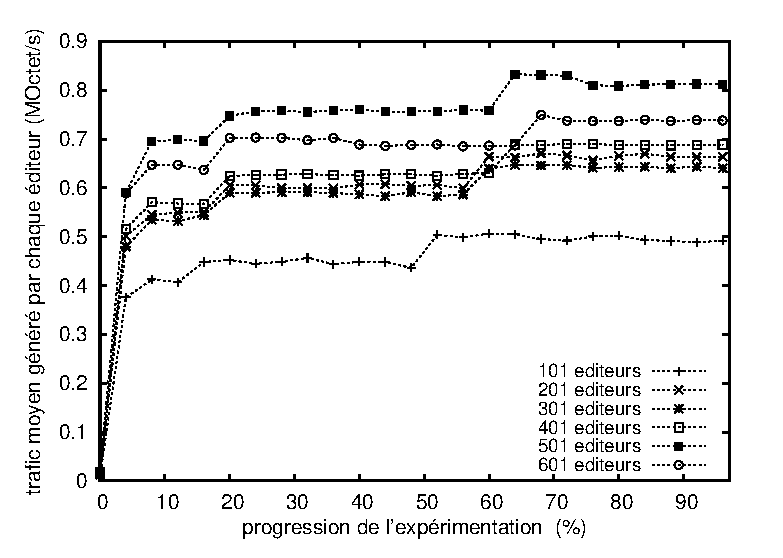
\includegraphics[width=1\textwidth]{img/editor/communication.eps}
  \end{center}

\end{frame}